\begin{tabular}{C{.2\textwidth} L{.71\textwidth}}
    
\includegraphics[width=\linewidth]{img/logos/qt.png}\captionsetup{width=\linewidth}\captionof{figure}{Logo de Qt.}\label{img:qt:logo} & \textit{Qt} est un framework\definition{Ensemble de composants logiciels permettant le développement d'un programme} permettant très facilement de créer des applications à interface graphique. \textit{Qt} est écrit en C++ mais dispose aussi de son propre langage de conception, \textit{QtQuick}. Son utilisation permet de développer des applications ou programmes à interface graphique sur plusieurs plateformes, telles que Windows, Linux et macOS pour n'en citer que quelques uns. L'un des gros avantages de \textit{Qt} qui fut également utilisé dans ce projet fut le système de connections de type \textit{Signal-Slot} que Qt propose.
\end{tabular}

Ce système de 'connexion' de composants permet d'établir facilement des relations de cause à effet pour les actions effectuées par l'utilisateur, le programme lui-même ou le système d'exploitation sous-jacent au programme. En effet, cette fonctionnalité de \textit{Qt} est une système de méta-programmation permettant de relier dynamiquement au temps d'exécution les actions d'un composant (qu'il soit à l'écran ou interne au programme) à une fonction spécifique d'un objet du même programme. Par exemple, si une valeur définie par un curseur change, il serait possible de mettre à jour une variable précedemment 'reliée' à ce curseur via une fonction de mise à jour comme \texttt{updateValue()}. Ci-dessous, vous trouverez un diagramme montrant le fonctionnement général du système. Étant donné que \textit{Qt} est multi-plateforme, ce système nous permet de nous abstraire du fonctionnement particulier du système d'exploitation sous-jacent au programme, afin de pouvoir mettre en place une architecture et un mode de fonctionnement dynamique pour le programme peu importe la plateforme choisie.

Ce système est utilisé dans la majorité des programmes, particulièrement dès lors qu'un contexte OpenGL est nécessaire. En effet, \textit{Qt} propose plusieurs composants afin de faciliter la création et la gestion des contextes OpenGL, ainsi que plusieurs classes permettant de faires diverses opérations sur ce contexte\footnote{Un contexte OpenGL est une instance depuis laquelle nous pouvons appeler des fonctions reliées à OpenGL. Plus d'informations dans l'annexe sur OpenGL}. De plus, ce système est utilisé pour contrôler les champs et boutons liés aux générations de grille, ainsi que les curseurs liés à la définition des plans de coupe.

L'un des avantages du système \textit{Slot-System} est le fait de pouvoir dynamiquement, à l'exécution du programme, redéfinir les connexions effectuées entre composants. Ainsi, il est possible de modifier le mode de fonctionnement d'un élément graphique sans en changer l'apparence par exemple.

\begin{figure}[ht]
    \centering
    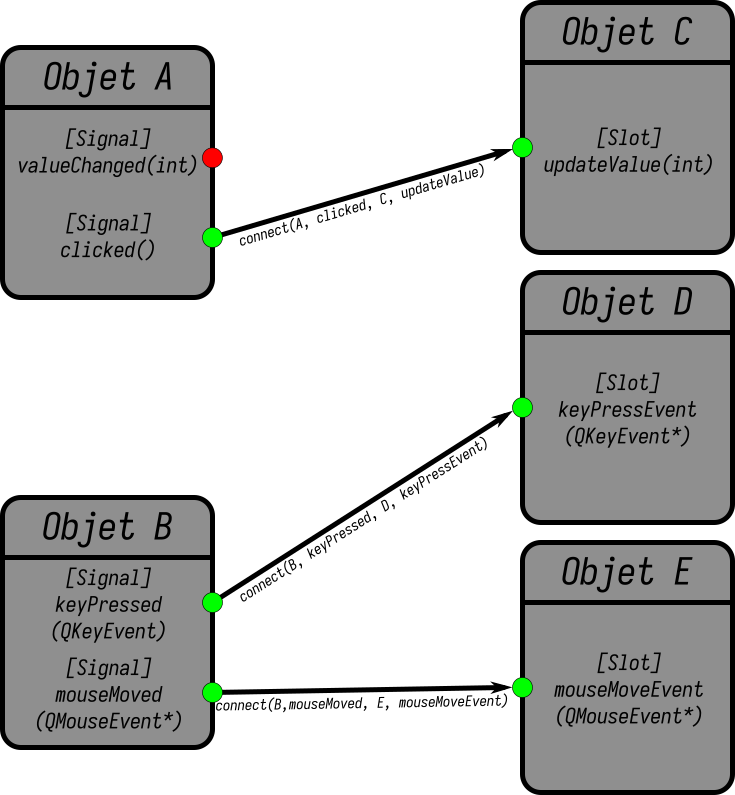
\includegraphics[width=.8\linewidth]{img/qt_slot_signal_diagram.png}
    \captionsetup{width=.8\textwidth}
    \caption{Le système de \textit{Signal-Slot} de \textit{Qt}. En vert, les signaux ou slots connectés, en rouge ceux non connectés.}
    \label{img:qt:signal_slot_diagram}
\end{figure}
